% https://tex.stackexchange.com/a/447344
\documentclass{beamer}
\usepackage[utf8]{inputenc}
\usetheme{Singapore}
\usepackage{tikzpeople,tikz}
\setbeamertemplate{navigation symbols}{}
\usetikzlibrary{positioning,shapes,calc,arrows}
\definecolor{gruen}{RGB}{18,133,66}
\definecolor{hell}{RGB}{55,181,74}
\tikzset{
    dollar/.style={
        append after command={
            \pgfextra{
                \node[draw,minimum width=1cm,minimum height=.5cm] (a) at (\tikzlastnode)
                {};
                \fill[gruen] (a.north west) rectangle (a.south east);
                \fill[white,radius=.04] ([xshift=.1cm,yshift=-.1cm]a.north west) circle;
                \fill[white,radius=.04] ([xshift=.1cm,yshift=.1cm]a.south west) circle;
                \fill[white,radius=.04] ([xshift=-.1cm,yshift=.1cm]a.south east) circle;
                \fill[white,radius=.04] ([xshift=-.1cm,yshift=-.1cm]a.north east) circle;
                \fill[hell] ([xshift=-.1cm,yshift=.2cm]a.south east) arc(90:180:.1) -- ([xshift=.2cm,yshift=.1cm]a.south west) arc(0:90:.1) -- ([xshift=.1cm,yshift=-.2cm]a.north west) arc(270:360:.1) -- ([xshift=-.2cm,yshift=-.1cm]a.north east) arc(180:270:.1) -- cycle;
                \fill[gruen,radius=.1cm] ($(a.north west)!.5!(a.south east)$) circle;
                \node[white] at ($(a.north west)!.5!(a.south east)$) {\tiny\sf\$};
            }
        }
    }
}
\begin{document}
    \begin{frame}
    \transduration<0-9>{0.1}
        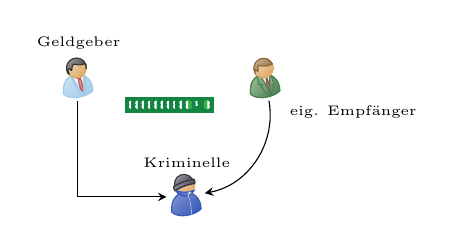
\begin{tikzpicture}[>=stealth,scale=2]
            \node[yshift=-.5cm,label=above:{\tiny Geldgeber},dave] (dave) {};
            \node[label=below right:{\tiny eig. Empfänger},businessman,right=2 of dave] (businessman) {};
            \node[label=above:{\tiny Kriminelle},criminal,right=1 of dave,yshift=-1.5cm] (criminal) {};
            \draw[->] (dave) |- (criminal);;
            \draw[<-] (criminal) to[bend right=45] (businessman);
            \foreach \x in{1,1.1,...,2}{
                \scalebox{.4}[.4]{\node<+>[dollar] at (\x,-1.05) {};}
            }
        \end{tikzpicture}
    \end{frame}
\end{document}
